@% Chapter 5

\chapter{Aplicação} % Main chapter title
\label{chap:Chapter5} % For referencing the chapter elsewhere, use \ref{chap:Chapter5} 

%----------------------------------------------------------------------------------------
\section{Sistema Desenvolvido}
O objetivo principal da parte prática da dissertação é não só recolher sinais e criar a sua função de ambiguidade, mas principalmente detetar um objeto estático e em movimento.
Para realizar estas tarefas foi utilizado um transmissor e recetor LimeSDR USB. As suas principais caraterísticas estão apresentadas na seguinte tabela e a sua documentação em \url{https://wiki.myriadrf.org/LimeSDR-USB}.\par

\begin{table}[h]
\centering
\begin{tabular}{@{}ccccc@{}}
\toprule
Caraterística       			 & Descrição                      \\ \midrule
\textit{RF Transreceiver}        & LMS7002M                       \\
\textit{Oscillator}    			 & Rakon RPT7050A @30.72$MHz$    \\
Banda de frequência              & 100$kHz$ - 3.8$GHz$            \\ 
Largura de banda máxima          & 61.44$MHz$                     \\ \bottomrule
\label{tab:limesdr}
\end{tabular}
\caption[Caraterísticas do LimeSDR USB]{Caraterísticas do LimeSDR USB}
\end{table}

Por forma a reduzir o ruído a alimentação é feita através dum \textit{power bank} de 20000$mAh$. Isto é conseguido com um cabo em "Y" que vem com o LimeSDR, que separa a entrada de dados da alimentação do equipamento.\par 
As duas antenas utilizada tanto para o canal de receção do sinal direto como do sinal refletido são antenas \textit{One for all} \textit{Yagi} de exterior para televisão, com $24dB$.\par 
Para a ligação entre o \textit{LimeSDR} e as antenas foram utilizados cabos coaxiais RG-58 com $1m$ de comprimento onde foram cravadas fichas SMA, como representado na figura \ref{fig:limec}.\par 
O repositório que contém as drivers que permitem trabalhar com o LimeSDR a partir do MATLAB foram desenvolvidos inicialmente e disponibilizado no link \url{https://github.com/jocover/Simulink-MATLAB-LimeSDR} em Agosto de 2017 pelo autor Jocover, posteriormente adaptado e atualizado em Dezembro de 2019 pelo autor Damir Rakhimov para a versão do LimeSuite 19.04 e pode ser acedido no \textit{github} do mesmo, \url{https://github.com/RakhDamir/LimeSDR-Matlab}. Todos os passos de instalação e configuração do sistema encontram-se disponibilizados no seu \textit{github}.

\begin{figure}[h]
\centering
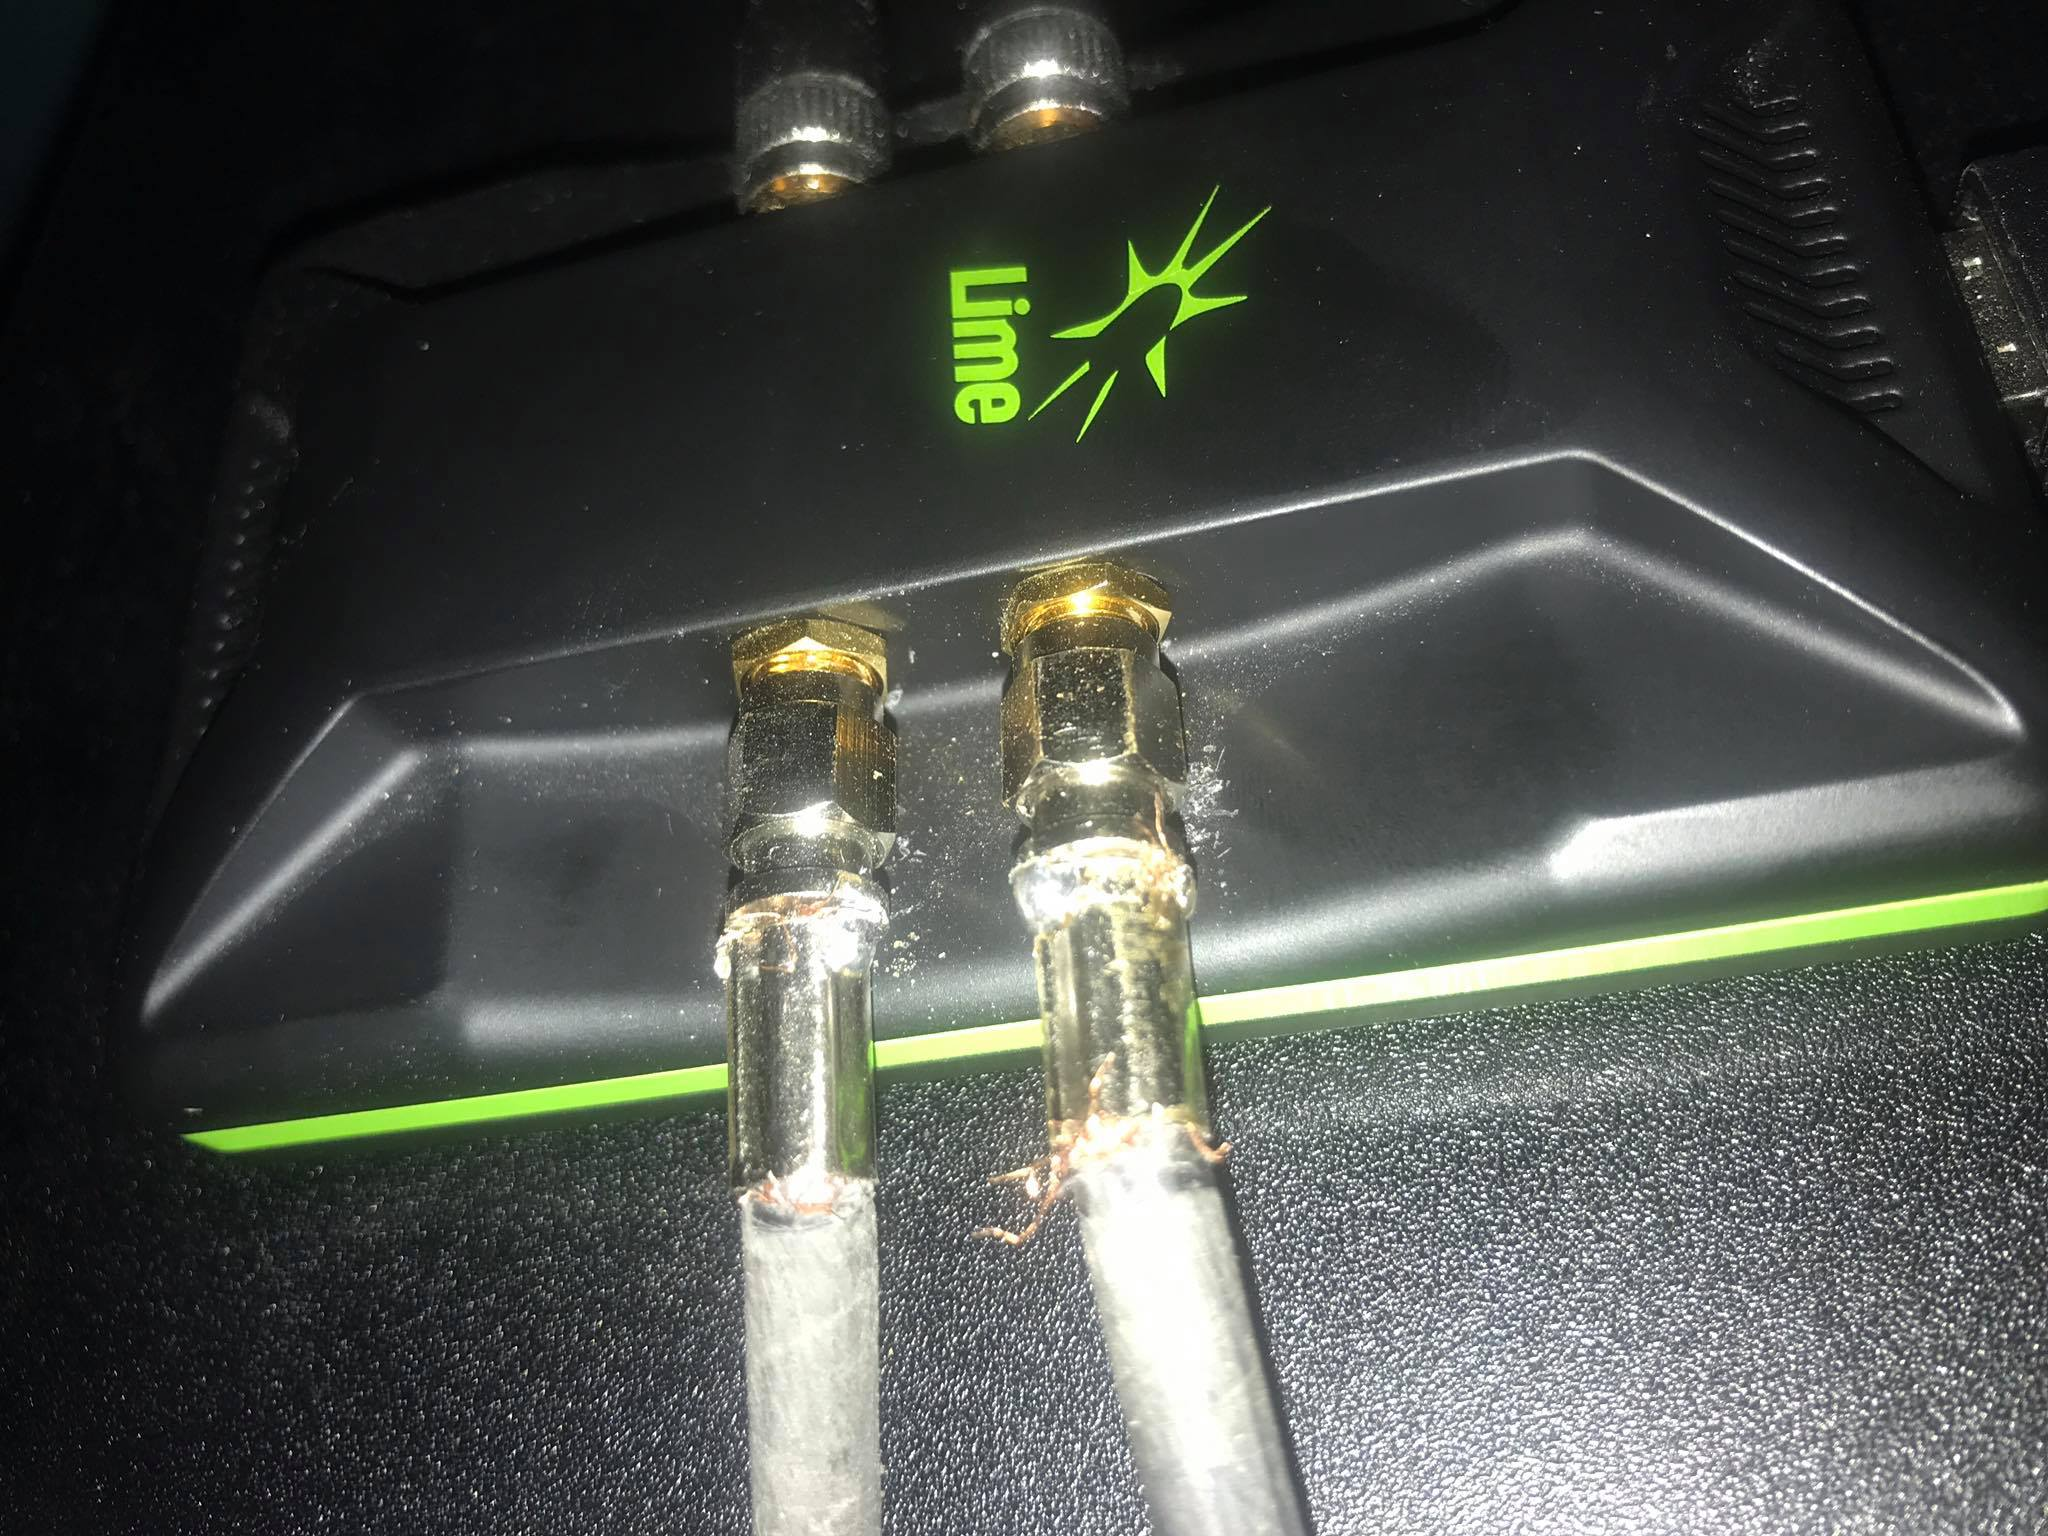
\includegraphics[scale=0.15]{chapters/ch5/assets/limec}
\caption[Entrada LimeSDR]{Entrada LimeSDR}
\label{fig:limec}
\end{figure}

Para o estudo da deteção de alvos utilizando sistemas de deteção passivos, foi utilizado sinais \gls{DVB-T} dos transmissores de Palmela (38°33'23.02"N	8°54'27.56"W) e Cruz de Pau (38°37'3.78"N	9°7'2.31"W), ambos a transmitir nas frequências $598-606 MHz$, e a posição do estudo foi em Brejos de Azeitão (38°32'11.10"N	9°1'21.43"W). Os sinais \gls{DVB-T} são de grande interesse para a deteção com radares passivos como abordado no Capítulo \ref{chap:Chapter1}, visto que entre os disponíveis como iluminadores de oportunidade apresentam uma boa cobertura e uma boa largura de banda, o que se reflete numa boa resolução em alcance. Para uma melhor compreensão do panorama geográfico, a imagem \ref{fig:mapaemi} representa os transmissores a amarelo,  os utilizados a amarelo com um risco preto por baixo e a posição da experiência com um círculo azul.\par 

\begin{figure}[h]
\centering
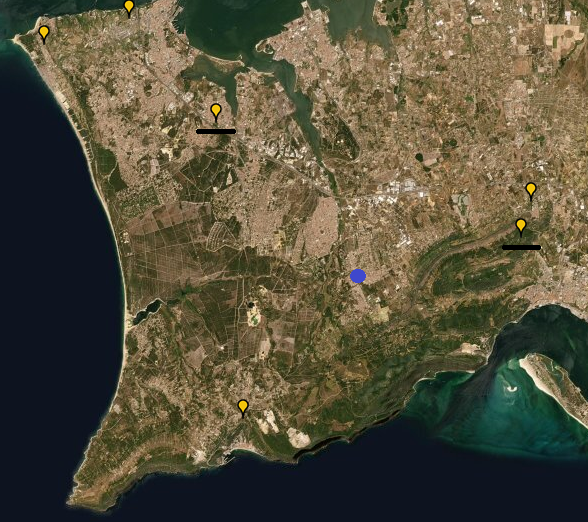
\includegraphics[scale=0.75]{chapters/ch5/assets/mapaemi}
\caption[Mapa de emissores e local da experiência]{Mapa de emissores e local da experiência}
\label{fig:mapaemi}
\end{figure}

Nesta experiência, a antena que recebe o sinal direto estava direcionada para Palmela, recebendo também sinal direto do transmissor da Cruz de Pau devido à pouca diretividade da antena, enquanto a antena que recebe o sinal refletido estava posicionada de modo a apontar noutra direção, como na figura \ref{fig:prat}. Recordando o Capítulo \ref{chap:Chapter3}, chegou-se à conclusão de que as duas antenas ao estarem em sentidos opostos, os lóbulos posteriores iam receber muito sinal indesejado, então mudou-se a geometria da experiência para evitar este problema.

\begin{figure}[h]
\centering
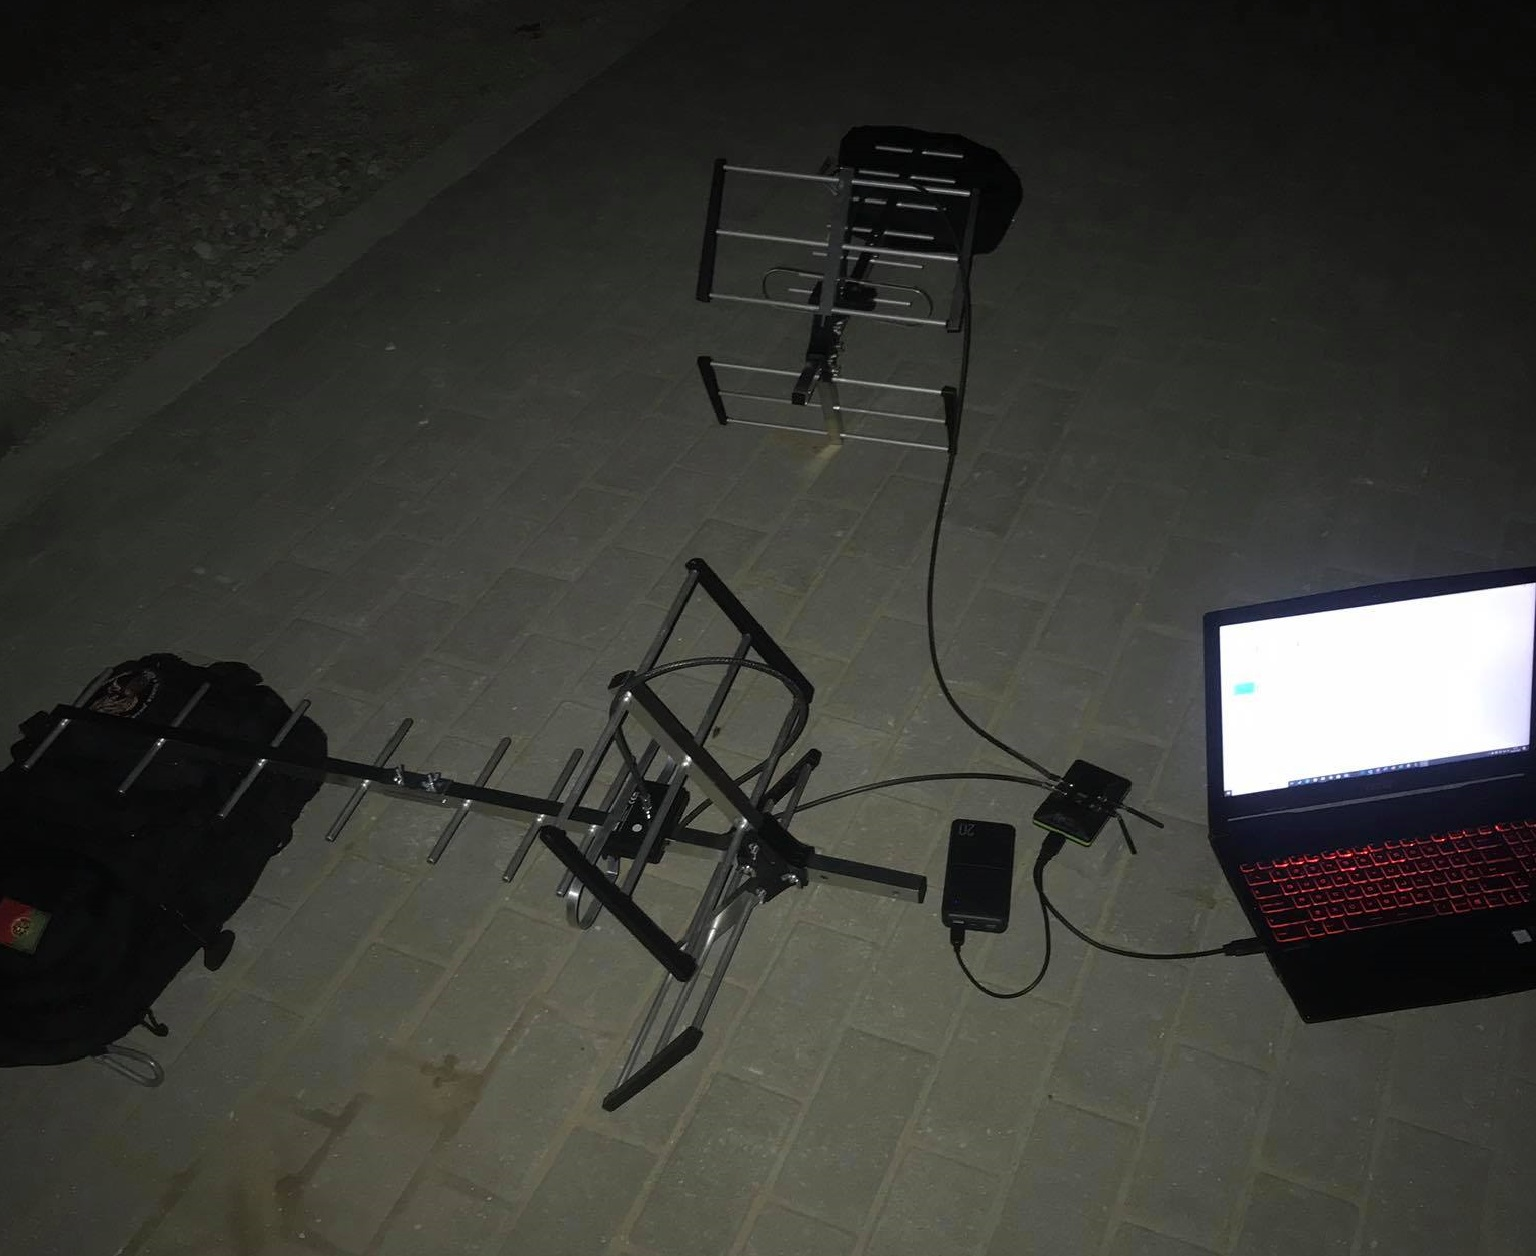
\includegraphics[scale=0.25]{chapters/ch5/assets/prat2}
\caption[Disposição do sistema]{Disposição do sistema no local da experiência}
\label{fig:prat}
\end{figure}

Antes de apresentar os resultados, é necessário compreender a situação em que se está inserido e as limitações do equipamento para se conseguir tirar conclusões coerentes. Com isto, os dois parâmetros a serem considerados inicialmente é a resolução em \textit{Doppler} e em alcance. Da expressão \ref{2.3}, é dada a resolução em alcance para o caso bistático. Visto que o ângulo $\beta$, entre o transmissor e o recetor toma valores perto dos $0^{\circ}$, o termo $cos\left( \dfrac{\beta}{2}\right) = 1$, logo, reduz-se ao caso monostático, e obtém-se o resultado em \ref{5.1}.

\begin{equation} \label{5.1}
\delta_{r}=\dfrac{c}{2B\left( cos\dfrac{\beta}{2}\right)}=\dfrac{3\cdot 10^{8}}{2\times 8\times 10^{6} \left( cos\dfrac{0}{2}\right)}=18.75 m
\end{equation}

Portanto, teoricamente, não é possível distinguir dois alvos com uma distância entre eles menor que $18.75 m$, e logicamente se o alvo estiver em movimento só irá ser detetado a mudança de célula de resolução a cada $18.75 m$.\par 

No caso do desvio de \textit{doppler}, a resolução é dada pela expressão \ref{2.7}, para o caso do recetor estático e alvo em movimento. Desta, para as mesmas condições acima definidas e um tempo de integração de $1 s$, resulta uma resolução em \textit{Doppler} de $2.5 m/s$. No entanto, com um frequência de amostragem utilizada de $17 MHz$ os cálculos são computacionalmente demasiado pesados para o \textit{Matlab} conseguir calcular, para qual a solução ótima seria a aplicação de algoritmos por forma a reduzir este peso, mas a utilizada foi a redução das amostras utilizadas para valores inferiores a $0.1\% $. Isto tem como consequência a diminuição do tempo de integração para $0.1\% \times 1s$ e o agravamento da resolução em \textit{Doppler} para valores extremamente elevados, na ordem das centenas de $m/s$.

\begin{equation} \label{5.2}
\Delta v = \dfrac{\dfrac{3\times 10^{8}}{602\times 10^{6}}}{2\times 1} = 0.25 m/s
\end{equation}



\section{Resultados}
Considerando todas as condições descritas acima para a realização da experiência, os resultados permitiram a deteção do alvo mas com muitas condicionantes, tornando o sistema de baixo custo muito limitado, o que era de esperar.\par  
Todas as amostras foram retiradas com o sistema descrito anteriormente e utilizando o programa no Apêndice \ref{AppendixB}. Inicialmente são introduzidos os parâmetros em variáveis e depois de aberto o \textit{LimeSDR} com o comando \textit{dev = limeSDR()} são inseridos nos dois canais de receção, rx0 e rx1, com a adição do \textit{dev.rx0.antenna = 2} que indica que o \textit{low noise amplifier} a ser utilizados pelo \textit{LimeSDR} é o LNAL, adequado para frequências entre os $0 - 2000 MHz$. Posteriormente os parâmetros são lidos depois de introduzidos para haver registo e verificar se correspondem ao desejado e também é feita a leitura da temperatura do dispositivo visto que este tem tendência a aquecer rapidamente e isto afeta a sua \textit{performance}. De seguida são criadas as matrizes de zeros que vão alojar o sinal recebido, são autorizados os parâmetros nos canais e calibrados os canais de receção para a frequência desejada. Com isto, é iniciado a recolha de dados dos dois canais ao mesmo tempo com o comando \textit{dev.start()} de modo a que as unidades de tempo batam certo nas duas amostras, o que é crucial para que os resultados sejam fidedignos. Durante o tempo de recolha que termina com o comando \textit{dev.stop()}, o sistema vai recolher $Fs*Ts$ amostras no canal 0 e 1 para as variáveis \textit{samples} e \textit{samples1}. Posto isto, é necessário reduzir o numero de amostras para se conseguir fazer a correlação sem que o MATLAB fique sem memória e de seguida, utilizando a função \textit{ambgfun} consegue-se fazer as funções de ambiguidade tanto como a correlação entre os dois sinais recebidos $x$ e $x1$. Finalmente são desenhados os espectro-gramas  dos sinais recebidos tanto como as suas funções de ambiguidade e a correlação.\par 

\begin{figure}[h]
\centering
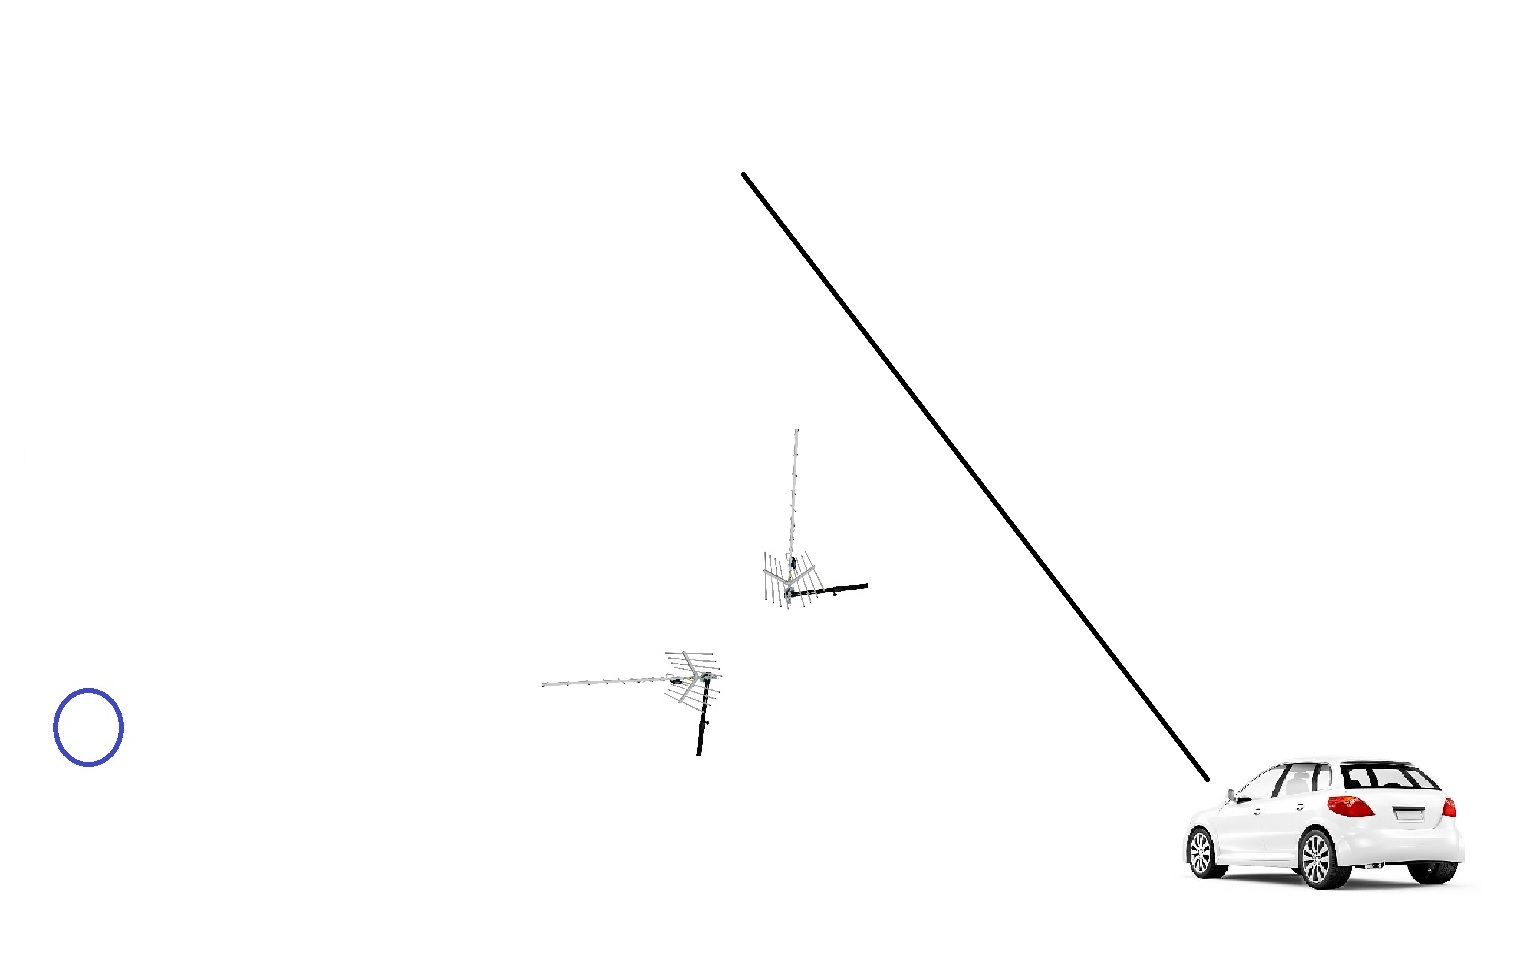
\includegraphics[scale=0.3]{chapters/ch5/assets/geoexp}
\caption[Configuração da experiência]{Configuração da experiência no local}
\label{fig:geoexp}
\end{figure}

A experiência foi dividia em 2 medições:
\begin{itemize}
\item Na primeira, um carro foi metido a $1 5m$ parado com um tempo de integração de $0.2 s$ (figura \ref{fig:15me});
\item No segundo caso, aumentou-se o tempo de integração para $2 s$ e fez-se passar o carro a uma velocidade de aproximadamente $40 km/h$ com uma posição inicial a $15m$ da antena que recebe o sinal refletido e passando a 
$1 m$ desta na sua posição mais próxima, como observável na figura \ref{fig:geoexp}(figura \ref{fig:15mm} e \ref{fig:15mmsum}). 
\end{itemize}

A janela escolhida para o \textit{Delay}, vai do valor $-3\times 10^{-7}$ a $3\times 10^{-7}$, o que segundo a expressão \ref{5.3} onde $t$ representa o \textit{delay} corresponde ao intervalo de $-45 m$ a $45 m$ e cada unidade representa $15 m$. Para a escala de \textit{Doppler}, segundo a expressão \ref{5.4}, para a frequência utilizada, cada $10 m/s = 36 km/h$ representa um desvio em \textit{doppler} de $20 Hz$.

\begin{equation} \label{5.3}
Range = \dfrac{c\times t}{2}
\end{equation}

\begin{equation} \label{5.4}
f_{d} = \dfrac{v}{c}f_{0}
\end{equation}

\begin{figure}[h]
\centering
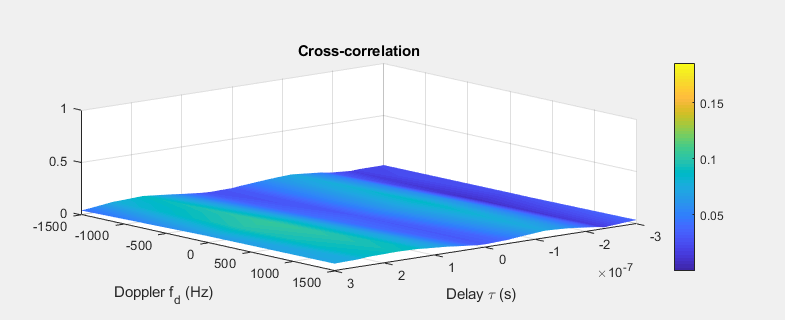
\includegraphics[scale=0.5]{chapters/ch5/assets/15me}
\caption[Caso 1]{Resultado do caso 1}
\label{fig:15me}
\end{figure}

Neste primeiro caso, verificamos a presença do carro na zona do $-1\times 10^{-7}s$ que se extende desde $-0.5\times 10^{-7}s$ a $-2\times 10^{-7}s$ que pode ser justificado com a resolução em alcance calculada com o valor de aproximadamente $19 m$ correspondente a aproximadamente $1.2\times 10^{-7} s$. O facto da frequência estar estendida para valores muito altos tem que ver não só com a resolução em \textit{Doppler} ser muito inadequada, mas maioritariamente pelo desalinhamento na amostragem dos dois canais de receção. Apesar de existir um comando que inicie ao mesmo tempo, o equipamento tem um defeito que desalinha a receção dos dois canais consoante o tempo de integração e a frequência, sendo que quanto maior valor estes tomarem, maior desvio haverá.

\begin{figure}[h]
\centering
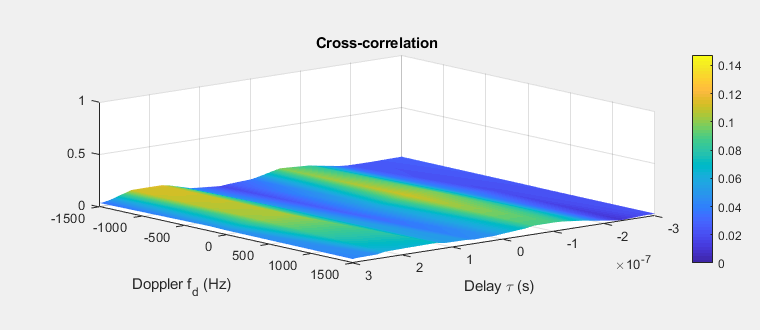
\includegraphics[scale=0.5]{chapters/ch5/assets/15mm}
\caption[Caso 2]{Resultado do caso 2}
\label{fig:15mm}
\end{figure}

Ao analisar o segundo caso, pode-se observar que por aumentar o tempo de integração, aumenta a intensidade da correlação de um alvo em relação às zonas onde não existe correlação.


\begin{figure}[h]
\centering
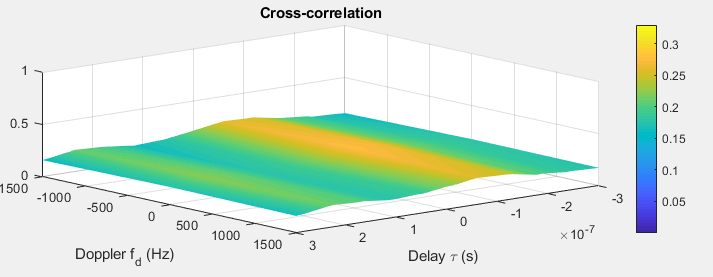
\includegraphics[scale=0.5]{chapters/ch5/assets/15mmsum}
\caption[Caso 2 especial]{Resultado do caso 2 com soma das amostras em diversas partes da matriz}
\label{fig:15mmsum}
\end{figure}

Ainda com os valores do segundo caso, mas somando amostras de diversas partes da matriz, é possível aumentar a intensidade da correlação no alvo se estivermos a utilizar zonas em que o carro se encontrava a refletir mais energia, ou seja, casos em que o carro estivesse mais perto e dentro da zona do diagrama de radiação da antena que tem maior intensidade. Para isto, foram usados os dados gravados do caso 2 e utilizado um programa no Apêndice \ref{AppendixC} que permite escolher as amostras de tempo da matriz que se querem analisar e fazer a correlação em cada uma delas. Uma forma de obter o valor de tempo em que o carro esteve mais perto do sistema é fazer uma correlação apenas em \textit{delay} e ver para que tempo a intensidade é máxima. No caso 2 obteve-se o valor de $0.9 s$ como o tempo em que o carro esteve mais próximo do radar, como se pode observar na figura \ref{fig:4ca}.

\begin{figure}[h]
\centering
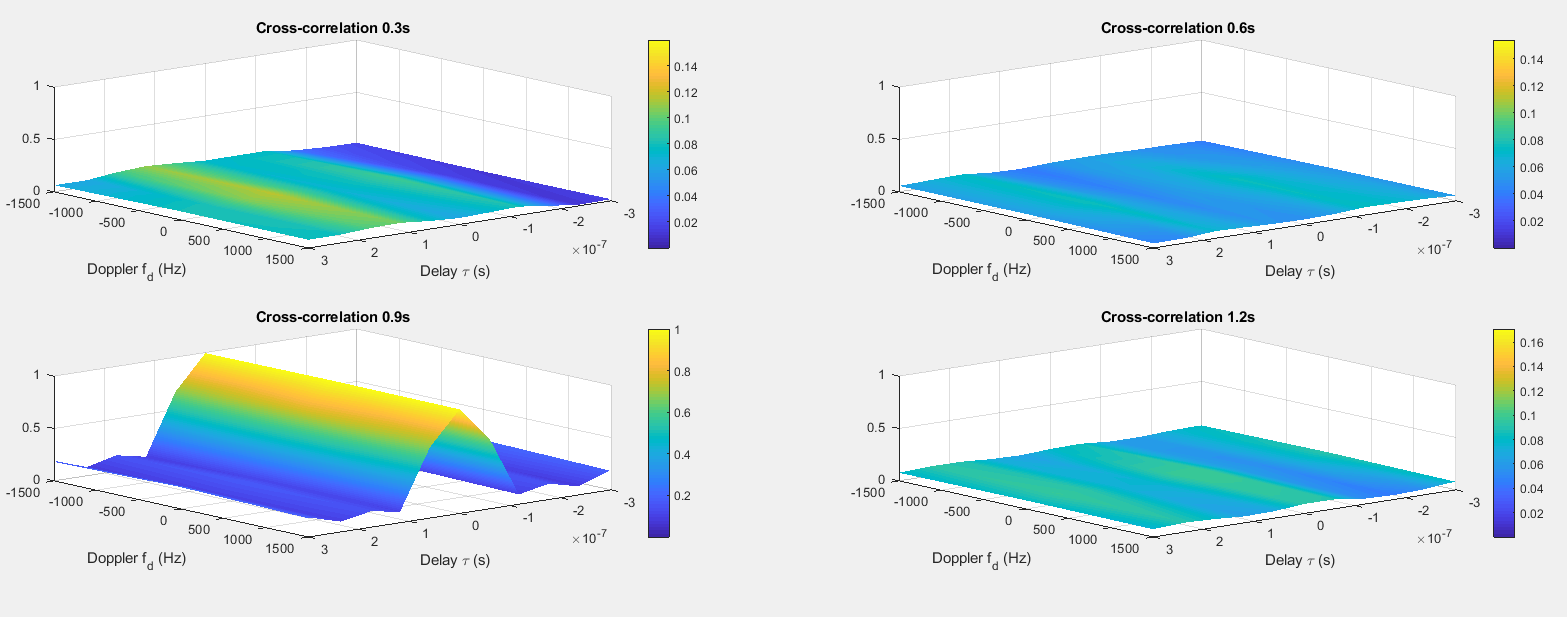
\includegraphics[scale=0.35]{chapters/ch5/assets/4ca}
\caption[Caso 2 dividido em 4 correlações]{Caso 2 dividido em 4 correlações, para $t=0.3s, 0.6s, 0.9s, 1.2s$}
\label{fig:4ca}
\end{figure}
